% !TEX root = handbook-physics.tex
%!TEX TS-program = pdflatex
%!TEX encoding = UTF-8 Unicode

\chapter{Gravitation}
\label{ch-06}
\zhtitle{万有引力}

\section{Law of Universal Gravitation}
\label{sec-6.1}
\zhtitle{万有引力定律}
\subsection{}\label{6.1.1} \redem{Isaac Newton's law of universal gravitation} states that the force of mutual attraction between any two particles is directly proportional to the product of their masses and inversely pro­portional to the square of the distance between them. Such forces are called \redem{gravitational forces}. If $m_{1}$ and $m_{2}$ are the masses of the particles being considered and $\vb{r}_{1}$ and $\vb{r}_{2}$ are the radius vectors of these particles, then, according to the law of univer­sal gravitation, the force $\vb{F}_{12}$ attracting the first particle toward the second particle, and the force $\vb{F}_{21}$ attracting the second particle toward the first particle are equal in magnitude and opposite in direction; they are equal to:
\zhpar{\redem{艾萨克·牛顿的万有引力定律}指出：任意两个质点之间的相互吸引力与两者质量的乘积成正比，与两者间距离的平方成反比。这种力称为\redem{引力}。设所考虑的两个质点的质量分别为 $m_{1}$ 和 $m_{2}$，其位矢分别为 $\vb{r}_{1}$ 和 $\vb{r}_{2}$，则根据万有引力定律，将第一个质点吸引向第二个质点的力 $\vb{F}_{12}$，与将第二个质点吸引向第一个质点的力 $\vb{F}_{21}$，大小相等、方向相反，其表达式如下式所示：}
\begin{equation*}%
\vb{F}_{12} = -G \frac{m_{1}m_{2}}{r_{12}^{3}} \vb{r}_{12} \,\,\textrm{and}\,\,\vb{F}_{21} = -G \frac{m_{1}m_{2}}{r_{21}^{3}} \vb{r}_{21}.
\end{equation*}
Here $\vb{r}_{12} = \vb{r}_{1} - \vb{r}_{2}$ and $\vb{r}_{21}= \vb{r}_{2} - \vb{r}_{1}$ are radius vectors from the second particle to the first and from the first to the second, respectively, and $r_{12} = r_{21}= \abs{\vb{r}_{12}}= \abs{\vb{r}_{21}}$ is the distance between the particles. 
\zhpar{式中 $\vb{r}_{12} = \vb{r}_{1} - \vb{r}_{2}$ 和 $\vb{r}_{21}= \vb{r}_{2} - \vb{r}_{1}$ 分别为从第二个质点指向第一个质点、以及从第一个质点指向第二个质点的位矢，$r_{12} = r_{21}= \abs{\vb{r}_{12}}= \abs{\vb{r}_{21}}$ 为两质点之间的距离。}

The proportionality factor $G$ is called the \redem{constant of universal gravitation}, or the \redem{gravitational constant}. In value the gravitational constant is equal to the force of mutual attraction of two particles of unit mass with a distance of unit length between them. It has been found from experi­ments that
\zhpar{比例系数 $G$ 称为\redem{万有引力常量}，或称\redem{引力常量}。其数值等于两个单位质量的质点相距单位长度时的相互吸引力。由实验测得的 $G$ 值如下式所示：}
\begin{equation*}%
G = \SI{6.6720 \pm 0.0041d-11}{\newton\metre\squared\per\kilo\gram\squared}.
\end{equation*}
\subsection{}\label{6.1.2} The gravitational interaction of two bodies of arbitrary size and shape (\figr{fig-06-01}) is described by the equation
\zhpar{两个任意大小和形状物体之间的引力相互作用（见\figr{fig-06-01}）可由下式描述：}
\begin{equation*}%
\vb{F}_{12} = -G \int_{(V_{1})} \rho_{1} \dd V_{1} \int_{(V_{2})} \frac{\rho_{2}}{r_{12}^{3}} \vb{r}_{12} \dd V_{2},
\end{equation*}
where $\vb{r}_{12}$ is the radius vector from the infinitely small element $\dd V_{2}$ of volume of the second body to the infinitely small el­ement $\dd V_{2}$ of volume of the first body, $\rho_{1}$ and $\rho_{2}$ are the densities of the two elements, and integration is carried out throughout the whole volume of both bodies.
\zhpar{式中 $\vb{r}_{12}$ 为从第二个物体的无穷小体积元 $\dd V_{2}$ 指向第一个物体的无穷小体积元 $\dd V_{1}$ 的位矢，$\rho_{1}$ 和 $\rho_{2}$ 分别为两个体积元的密度，积分遍及两个物体的整个体积。}
\begin{figure}[H]
%\begin{wrapfigure}{r}{0.5\linewidth}
\centering
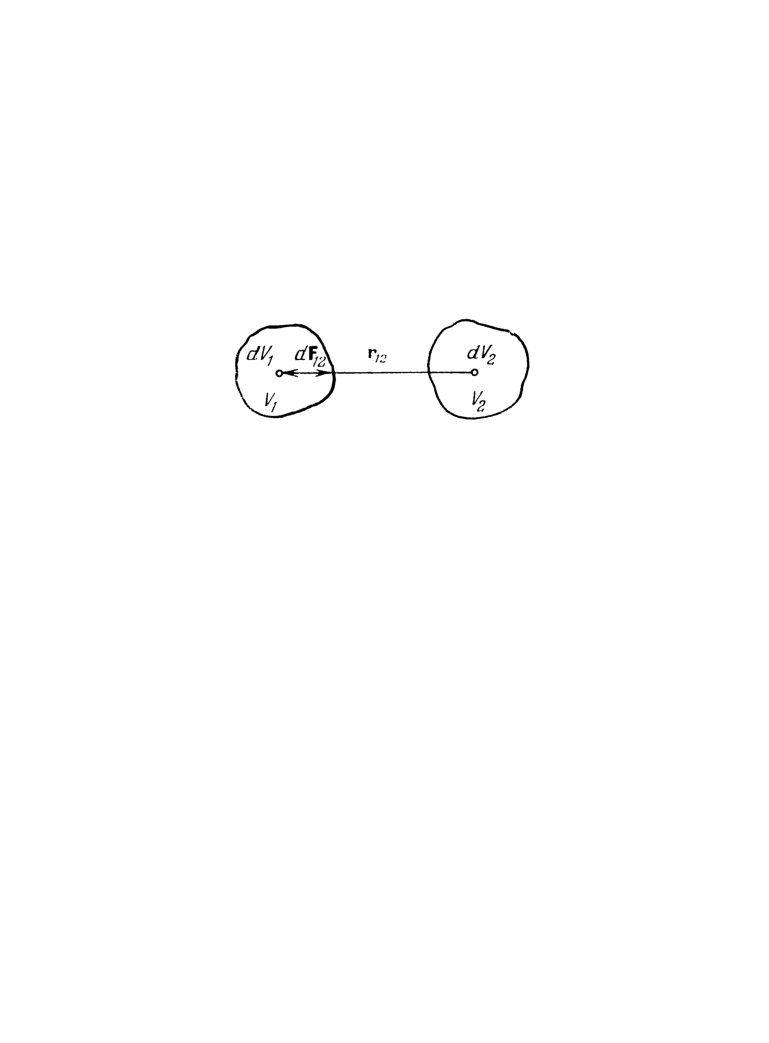
\includegraphics[width=0.7\textwidth]{figs/ch-06/fig-06-01.pdf}
%\input{figs/ch-03/fig-03-01}
%  \vspace{-13pt}
\sidecaption{The gravitational interaction between two bodies of arbitrary size and shape.\zhcap{两个任意大小和形状物体之间的引力相互作用。}\label{fig-06-01}}
\end{figure}
The calculations of force $\vb{F}_{12}$ are substantially simplified in two cases:
\zhpar{在以下两种情形下，$\vb{F}_{12}$ 的计算可以大大简化：}
\begin{enumerate}[label=(\alph*)]
\item when there is a spherically symmetrical distribution of the masses in the two bodies, i.e. both bodies are of spherical shape and the density of each body depends only upon the distance to its centre (in particular, the bodies can be homogeneous); \item when one of the bodies is of negligibly small size with respect to the other body in which the distribution of its mass is spherically symmetrical.
\zhpar{（a）两个物体中的质量呈球对称分布，即两物体均为球形，且每个物体的密度仅取决于到其球心的距离（特别地，物体可以是均匀的）；（b）其中一个物体的线度相对于另一物体可以忽略不计，且另一物体的质量呈球对称分布。}
\end{enumerate}
In these cases
\zhpar{在这些情形下，}
\begin{equation*}%
\vb{F}_{12} = -G \frac{m_{1}m_{2}}{r_{12}^{3}} \vb{r}_{12},
\end{equation*}
where $m_{1}$ and $m_{2}$ are the masses of the bodies, and $\vb{r}_{12}$ is the radius vector connecting the centres of mass \ssect{2.3.3} of the second and first bodies.
\zhpar{式中 $m_{1}$ 和 $m_{2}$ 为两物体的质量，$\vb{r}_{12}$ 为连接第二个物体与第一个物体质心的位矢（见\ssect{2.3.3}）。}

\subsection{}\label{6.1.3} As a first approximation, it can be assumed that the earth is of spherical shape and the distribution of its mass is spherical­ ly symmetrical. Hence the gravitational force $\vb{F}$, exerted by the earth on a body of mass $m$, is directed toward the centre of the earth and its magnitude is
\zhpar{作为第一级近似，可以认为地球为球形，且其质量呈球对称分布。因此，地球施于质量为 $m$ 的物体的引力 $\vb{F}$ 指向地心，其大小为}
\begin{equation*}%
F = G \frac{mM_{\Earth}}{r^{2}},
\end{equation*}
where $M_{\Earth}$ is the mass of the earth and $r$ is the distance from the body to the earth's centre (the size of any body on earth is negligibly small compared to the radius of the earth).
\zhpar{式中 $M_{\Earth}$ 为地球的质量，$r$ 为物体到地心的距离（地球上任何物体的线度与地球半径相比都可以忽略不计）。}

\subsection{}\label{6.1.4} In application to such microscopic objects as elementary particles, gravitational interaction is practically of no import­ance whatsoever. It is found to be extremely weak in comparison to all other kinds of interaction: strong, electromagnetic and weak interaction (\ssect{43.2.5} through \ssect{43.2.8}). For example, the electric force of mutual repulsion of two electrons exceeds their gravitational force by over \num{d42} times! Even for ordinary macro­scopic objects on the earth the forces of gravitational inter­ action are extremely small. Two homogeneous spheres, for instance, with a mass of \SI{1000}{\kilo\gram} each and a distance of one metre between their centres are attracted to each other with a force of only \SI{7d-5}{\newton}.
\zhpar{对于电子等基本粒子这类微观客体，引力相互作用实际上毫无重要性。与其他各类相互作用（强相互作用、电磁相互作用和弱相互作用，见\ssect{43.2.5}至\ssect{43.2.8}）相比，引力极其微弱。例如，两个电子之间的静电斥力比它们之间的引力大出 \num{d42} 倍以上！即使对于地球上的普通宏观物体，引力相互作用也极其微小。例如，两个质量各为 \SI{1000}{\kilo\gram}、球心相距一米的均匀球体，其相互吸引力仅为 \SI{7d-5}{\newton}。}

But, at the same time, gravitational forces are the determining factors in the motion of objects that are investigated in astron­omy and astronautics (spaceships, planets and their satellites, planetary systems, stars, etc.). This is due, primarily, to the huge size of astronomical bodies and, in the second place, to the small electromagnetic forces of interaction of such bodies, which, as a whole, are practically electroneutral.
\zhpar{但与此同时，引力却是天文学和宇宙航行学（宇宙飞船、行星及其卫星、行星系统、恒星等）所研究的物体运动的决定性因素。这首先是由于天体的尺度极其巨大，其次是由于这类天体的电磁相互作用很小，整体上实际是电中性的。}

\section{Gravitational Field}
\label{sec-6.2}
\zhtitle{引力场}

\subsection{}\label{6.2.1} Gravitational interaction between bodies is due to the \redem{gravitational field} set up by the bodies. A distinctive feature of a gravitational field is that a particle placed in this field is subject to a force proportional to the mass of the particle.
\zhpar{物体之间的引力相互作用是由物体所建立的\redem{引力场}产生的。引力场的一个显著特点是，置于其中的质点所受的力与该质点的质量成正比。}

The force characteristic of a gravitational field is its \redem{intensity}, the vector quantity $\vb{g}_{f}$, which is equal to the ratio of the force $\vb{F}$, exerted on the particle by the field in which it is placed, to the mass $m$ of the particle:
\zhpar{描述引力场的特征量是其\redem{场强}，它是一个矢量 $\vb{g}_{f}$，等于场作用于置于其中的质点的力 $\vb{F}$ 与该质点质量 $m$ 之比：}
\begin{equation*}%
\vb{g}_{f} = \frac{\vb{F}}{m}.
\end{equation*}
The intensity of a gravitational field is independent of the mass $m$ of the particle. It is a function of the coordinates $(x, \,y,\, z)$ of points of the field being considered. In the case of an unsteady field the intensity also depends upon the time $t$.
\zhpar{引力场的场强与质点的质量 $m$ 无关，它是所考虑场中各点坐标 $(x, \,y,\, z)$ 的函数。对于非定常场，场强还与时间 $t$ 有关。}

A gravitational field is steady, or stationary \ssect{2.2.1}, if the body that sets it up is fixed in the frame of reference chosen to describe the field. The intensity of a steady gravitational field depends only upon the coordinates: $\vb{g}_{f} = \vb{g}_{f} (x,\, y,\, z)$.
\zhpar{若产生引力场的物体在描述该场的参考系中是静止的，则该引力场是定常的，或称稳恒的（见\ssect{2.2.1}）。定常引力场的场强仅依赖于坐标：$\vb{g}_{f} = \vb{g}_{f} (x,\, y,\, z)$。}

It follows from Newton's second law \ssect{2.4.3} that the forces of ;i gravitational field impart an acceleration $\vb{a}$ to a free particle in the field. This acceleration equals the intensity of the field:
\zhpar{由牛顿第二定律（见\ssect{2.4.3}）可知，引力场的作用力使场中的自由质点获得加速度 $\vb{a}$。该加速度等于场强：}
\begin{equation*}%
\vb{a} = \frac{\vb{F}}{m} = \vb{g}_{f}.
\end{equation*}

\subsection{}\label{6.2.2} It follows from the law of universal gravitation \ssect{6.1.1} that the intensity of the gravitational field of a fixed particle of mass $M$, located at the origin of coordinates, equals
\zhpar{由万有引力定律（见\ssect{6.1.1}）可知，位于坐标原点的静止质点（质量为 $M$）的引力场场强为}
\begin{equation*}%
\vb{g}_{f} = - G \frac{M}{r^{3}} \vb{r},
\end{equation*}
where $\vb{r}$ is the radius vector of the point being considered in the field.
\zhpar{式中 $\vb{r}$ 为场中所考虑点的位矢。}

A gravitational field is a conservative, or potential, one \ssect{3.1.6} because the force acting on a particle of mass m brought into the field is a central force \ssect{3.3.4}:
\zhpar{引力场是保守场，或称有势场（见\ssect{3.1.6}）。这是因为置于其中的质量为 $m$ 的质点所受的力是有心力（见\ssect{3.3.4}）：}
\begin{equation*}%
\vb{F} = m\vb{g}_{f} = - G \frac{mM}{r^{2}} \frac{\vb{r}}{r}.
\end{equation*}
Correspondingly, the potential energy of a particle in such a field is equal to (3.3.4):\footnote{Here and throughout \sect{sec-6.2} and \sect{sec-6.3} an infinitely distant point is chosen as the reference point for the potential energy, i.e. it is assumed that $E_{p} (\infty) = 0$.}
\zhpar{相应地，质点在该场中的势能由（3.3.4）式给出：}
\zhpar{注：此处及整个 \sect{sec-6.2} 和 \sect{sec-6.3} 中，势能的参考点均取为无穷远点，即假定 $E_{p} (\infty) = 0$。}
\begin{equation*}%
E_{p} = \int_{r}^{\infty} F_{r} \dd r = -GmM \int_{r}^{\infty} \frac{\dd r}{r^{2}} = -G\frac{mM}{r}.
\end{equation*}
It is equally correct to regard the quantity $E_{p}$ as the potential energy of a particle of mass $M$ in a gravitational field set up by a particle of mass $m$ or, finally, as the \redem{mutual potential energy of two particles} due to their gravitational interaction.
\zhpar{同样正确的是，可以将量 $E_{p}$ 看作质量为 $M$ 的质点在质量为 $m$ 的质点所建立的引力场中的势能；或最终看作由于引力相互作用而具有的两质点的\redem{相互势能}。}

\subsection{}\label{6.2.3} A gravitational field complies with the \redem{principle of super­ position of fields}: in superposing several $(n)$ gravitational fields their intensities at each point in space are added vectorially, i.e. the intensity of the resultant field is
\zhpar{引力场服从\redem{场的叠加原理}：在叠加若干个（$n$ 个）引力场时，它们在空间各点的场强矢量相加，即合成场的场强为}
\begin{equation*}%
\vb{g}_{f} = \sum_{i=1}^{n} \vb{g}_{f\!i},
\end{equation*}
where $\vb{g}_{f\!i}$ is the intensity of only the $i$-th field at the point being considered in space.
\zhpar{式中 $\vb{g}_{f\!i}$ 为空间中所考虑点处仅由第 $i$ 个场产生的场强。}

The intensity of the gravitational field of an arbitrary system consisting of $n$ fixed particles is
\zhpar{由 $n$ 个固定质点组成的任意质点系的引力场场强为}
\begin{equation*}%
\vb{g}_{f} = - G \sum_{i=1}^{n} \frac{m_{i}}{\rho_{i}^{3}} \pmb{\rho}_{i},
\end{equation*}
where $\pmb{\rho}_{i} = \vb{r} - \vb{r}_{i}$ is the radius vector from the $i$-th particle, whose radius vector is equal to $\vb{r}_{i}$, to the point in the field spec­ified by radius vector $\vb{r}$. Consequently, the potential energy of a particle of mass $m$ in this gravitational field is
\zhpar{式中 $\pmb{\rho}_{i} = \vb{r} - \vb{r}_{i}$ 为从位矢为 $\vb{r}_{i}$ 的第 $i$ 个质点指向场中由位矢 $\vb{r}$ 确定的点的位矢。因此，质量为 $m$ 的质点在该引力场中的势能为}
\begin{equation*}%
E_{p} = - Gm \sum_{i=1}^{n} \frac{m_{i}}{\rho_{i}}.
\end{equation*}
In particular, if the gravitational field is set up by a body whose mass $M$ is distributed in a spherically symmetrical manner \ssect{6.1.2}, then outside this body
\zhpar{特别地，若引力场是由质量为 $M$ 且呈球对称分布的物体（见\ssect{6.1.2}）产生的，则在该物体外部}
\begin{equation*}%
\vb{g}_{f} = - G \frac{M}{r^{3}} \vb{r}\quad \textrm{and}\quad E_{p} = -\frac{GmM}{r},
\end{equation*}
where $\vb{r}$ is a radius vector from the centre of the body to the point being considered in the field. These equations are valid, for example, for the gravitational field of the earth.
\zhpar{式中 $\vb{r}$ 为从物体中心到场中所考虑点的位矢。例如，上述关系对地球的引力场是适用的。}

\subsection{}\label{6.2.4} By virtue of the conservative nature (potentiality) of the gravitational field \ssect{3.1.6}, its energy characteristic, the potential, ran be introduced. The \redem{potential of a gravitational field} is the scalar $\varphi$, equal to the ratio of the potential energy $E_{p}$of a par­ticle, placed at the point being considered in the field to the mass $m$ of the particle:
\zhpar{由于引力场是保守的（有势的），其能量特征量——势——可以引入。\redem{引力场的势}是一个标量 $\varphi$，它等于置于场中所考虑点处的质点的势能 $E_{p}$ 与该质点质量 $m$ 之比：}
\begin{equation*}%
\varphi = \frac{E_{p}}{m}.
\end{equation*}
The potential $\varphi$ is independent of the mass $m$ of the particle; it is a function of the coordinates of points of the gravitational, held. For example, the potential of a gravitational field set up by a fixed particle of mass $M$ is
\zhpar{引力场的势 $\varphi$ 与质点的质量 $m$ 无关，它是引力场中各点坐标的函数。例如，由位于固定点的质量为 $M$ 的质点所建立的引力场的势为}
\begin{equation*}%
\varphi = - \frac{GM}{r},
\end{equation*}
where $r$ is the distance from the source of the field to the point being considered.
\zhpar{式中 $r$ 为场源到所考虑点的距离。}

The potential of a gravitational field set up by an arbitrary system of $n$ fixed particles is
\zhpar{由任意 $n$ 个固定质点组成的质点系所建立的引力场的势为}
\begin{equation*}%
\varphi = - \sum_{i=1}^{n}G \frac{m_{i}}{\rho_{i}},
\end{equation*}
where $\rho_{i}$ is the distance from a particle of mass $m_{i}$ to the point being considered in the field. Thus, in superposing gravitational fields, their potentials are added together algebraically, i.e. the potential $\varphi$ at any point of a resultant field is equal to the algebraic sum of the potentials at the same point for all the superposed fields taken separately;
\zhpar{式中 $\rho_{i}$ 为质量为 $m_{i}$ 的质点到场中所考虑点的距离。因此，在叠加引力场时，各场的势代数相加，即合成场在任一点的势 $\varphi$ 等于各被叠加场在同一点单独考虑时的势的代数和，即}
\begin{equation*}%
\varphi = - \sum_{i=1}^{n} \varphi_{i}.
\end{equation*}
\hlblue{Note.} In applying this equation it is necessary that the same reference point be chosen for the potentials $\varphi_{i}$ of all the fields being superposed: $\varphi_{i}(\infty)=0$ (see the footnote to \ssect{6.2.2}). 
\zhpar{\hlblue{注意。}应用此式时，必须为所有被叠加场的势 $\varphi_{i}$ 选取相同的参考点，即 $\varphi_{i}(\infty)=0$（见\ssect{6.2.2}中的脚注）。}

\subsection{}\label{6.2.5} An element of work done by the forces of a gravitational field in an infinitely small displacement $\dd r$ of a particle of mass $m$ in this field is:
\zhpar{质量为 $m$ 的质点在该引力场中作无穷小位移 $\dd \vb{r}$ 时，引力场的力所做的功元为}
\begin{equation*}%
\dd W = (\vb{F} \,\dd \vb{r}) = m (\vb{g}_{f} \dd \vb{r}).
\end{equation*}
But, on the other hand, the work $\dd W$ is equal to the decrease in the potential energy of the particle in the gravitational field:
\zhpar{另一方面，功 $\dd W$ 等于质点在引力场中势能的减少量：}
\begin{equation*}%
\dd W = - \dd E_{p} = - m \dd \varphi.
\end{equation*}
Consequently, the potential and intensity of a gravitational field are related by the equation:
\zhpar{因此，引力场的势与场强之间满足下列关系：}
\begin{equation*}%
\dd \varphi = -(\vb{g}_{f} \dd \vb{r}) = -(g_{f\!x}\dd x + g_{f\!y}\dd y +g_{f\!z}\dd z),
\end{equation*}
where $g_{f\!x}$, $g_{f\!y}$ and $g_{f\!z}$ are the projections of vector $\vb{g}_{f}$ on the axes of rectangular Cartesian coordinates. Since
\zhpar{式中 $g_{f\!x}$、$g_{f\!y}$ 和 $g_{f\!z}$ 为矢量 $\vb{g}_{f}$ 在直角笛卡儿坐标轴上的投影。由于}
\begin{equation*}%
\dd \varphi = \pdv{\varphi}{x} \dd x + \pdv{\varphi}{y} \dd y + \pdv{\varphi}{z} \dd z,
\end{equation*}
then
\zhpar{则有}
\begin{equation*}%
\pdv{\varphi}{x}  = -g_{f\!x},\quad \pdv{\varphi}{y}  = -g_{f\!y},\quad\pdv{\varphi}{z}  = -g_{f\!z}.
\end{equation*}
Hence
\zhpar{由此得}
\begin{equation*}%
\vb{g}_{f}  = - \left(\pdv{\varphi}{x}\vu{i} +\pdv{\varphi}{y}\vu{j} + \pdv{\varphi}{z}\vu{k} + \right) = - \,\,\textrm{grad} \,\varphi = -\grad \varphi,
\end{equation*}
i.e. the intensity of a gravitational field is numerically equal and opposite in direction to the gradient of the potential of the field.
\zhpar{即引力场的场强在数值上等于场的势的梯度，方向相反。}

The relation between (p and gf can also be written in the form
\zhpar{$\varphi$ 与 $\vb{g}_{f}$ 之间的关系也可以写成下列形式：}
\begin{equation*}%
\dd \varphi = - \vb{g}_{f} \dd l \cos \alpha = -g_{f\!l} \dd l \quad \textrm{or} \quad g_{f\!l} = - \frac{\dd \varphi}{\dd l},
\end{equation*}
where $\alpha$ is the angle between vectors $\vb{g}_{f}$ and $\dd \vb{r}$, $\dd l = \abs{\,\dd \vb{r}\,}$, and $g_{f\!l}$ is the projection of vector $\vb{g}_{f}$ onto the direction of vec­tor $\dd \vb{r}$. Thus, the projection of the intensity vector of a gravita­tional field onto some direction is numerically equal and opposite in sign to the change in the field potential per unit length in the same direction.
\zhpar{式中 $\alpha$ 为矢量 $\vb{g}_{f}$ 与 $\dd \vb{r}$ 之间的夹角，$\dd l = \abs{\,\dd \vb{r}\,}$，$g_{f\!l}$ 为矢量 $\vb{g}_{f}$ 在 $\dd \vb{r}$ 方向上的投影。因此，引力场的场强矢量在某一方向上的投影，在数值上等于沿该方向单位长度上场的势的变化量，但符号相反。}

\subsection{}\label{6.2.6} The non-relativistic theory of gravitation discussed above end based on Newton's law of universal gravitation is only approximate. It describes with sufficient accuracy only comparatively weak gravitational fields, having a potential $\abs{\varphi}\ll c^{2}$, where $c^{2} = \SI{9e16}{\meter\squared\per\second\squared}$ is the square of the velocity of light in free space. It is, in particular, applicable to the gravitational lieIds of the earth and sun because the absolute values of the potentials of these fields at the surfaces of the earth and sun are equal to \num{6.3e7} and \SI{1.9e11}{\meter\squared\per\second\squared}.
\zhpar{上文所述基于牛顿万有引力定律的非相对论引力理论只是近似的。它仅能足够精确地描述较弱的引力场，即势满足 $\abs{\varphi}\ll c^{2}$ 的引力场，其中 $c^{2} = \SI{9e16}{\meter\squared\per\second\squared}$ 为真空中光速的平方。特别地，它适用于地球和太阳的引力场，因为这两个场在地球和太阳表面的势的绝对值分别等于 \num{6.3e7} 和 \SI{1.9e11}{\meter\squared\per\second\squared}。}

\subsection{}\label{6.2.7} The \redem{modern} (relativistic) \redem{theory of gravitation}, which is m unified theory of space, time and gravitation, was formulated by Albert Einstein. He called it the \redem{general theory of relativity}. The existence of a close relationship between space and time had already been indicated in his special theory of relativity. This relationship is evident in the Lorentz transformations \ssect{5.3.2} and the invariance of the interval between two events \ssect{5.4.8}. It was found necessary, in describing physical processes, l.o employ a four-dimensional space-time continuum, in which the position of a point is specified by three space coordinates mid the time coordinate $ct$.
\zhpar{现代（相对论性）引力理论是关于空间、时间与引力的统一理论，由阿尔伯特·爱因斯坦建立。他称之为\redem{广义相对论}。空间与时间之间的密切联系在他的狭义相对论中已经有所体现。这种关系表现在洛伦兹变换（见\ssect{5.3.2}）以及两事件间间隔的不变性（见\ssect{5.4.8}）之中。在描述物理过程时，有必要采用四维时空连续区，其中一点的位置由三个空间坐标和时间坐标 $ct$ 确定。}

According to the relativistic theory of gravitation, the geo­metrical properties (metric) of the space-time continuum depend upon the distribution of gravitating masses and their motion in space. Bodies setting up a gravitational field ``distort'' real three-dimensional space and differently change the passage of time at various points in this space. This means that the bodies cause a deviation of the metric of space-time from that of the ``flat'' space-time described by Euclidean geometry and dealt with in the special theory of relativity. Therefore, the motion of a body in a gravitational field can be regarded as inertial motion, but in a ``distorted'' (non-Euclidean) space-time continuum. Accordingly, a particle, subject to the action of a gravitational field, travels neither in a straight line nor at uniform velocity in a real three-dimensional space.
\zhpar{根据相对论性引力理论，时空连续区的几何性质（度规）取决于引力质量的分布及其在空间中的运动。产生引力场的物体使真实的三维空间“发生畸变”，并以不同的方式改变空间中各点的时间进程。这意味着，物体使时空的度规偏离了由欧几里得几何描述的“平直”时空度规（即狭义相对论所采用的度规）。因此，物体在引力场中的运动可以看作在“畸变”（非欧几里得）的时空连续区中的惯性运动。相应地，受引力场作用的质点，在真实的三维空间中既不沿直线运动，也不作匀速运动。}

It was shown in the relativistic theory of gravitation that the principle of superposition \ssect{6.2.3} does not hold for arbitrary gravitational fields. This principle, as well as the whole non-relativistic theory of gravitation, is sufficiently accurate only in weak fields $(\abs{\, \varphi \,} \ll c^{2})$ and for motion in these fields at low velocities $v \ll c$.
\zhpar{相对论性引力理论表明，叠加原理（见\ssect{6.2.3}）对任意引力场并不成立。这一原理以及整个非相对论引力理论，仅在弱场（$(\abs{\, \varphi \,} \ll c^{2})$）中以及物体在这些场中作低速运动（$v \ll c$）时，才具有足够的精确性。}


\clearpage

\section{Kepler's Laws. Space Velocities}
\label{sec-6.3}
\zhtitle{开普勒定律。宇宙速度}

\subsection{}\label{6.3.1} The motion of the planets of the solar system along their orbits around the sun complies with the three laws of Kepler. These laws can be derived from Newton's law of uni­versal gravitation, dealing, as a first approximation, with the sun and planets as particles. In the central force field of gravitation of the sun, a planet of mass $m$ is subject to the action of the gravitational force
\zhpar{太阳系行星沿其轨道绕太阳运动，遵循开普勒三定律。在第一级近似下，将太阳和行星视为质点，这些定律可由牛顿万有引力定律导出。在太阳引力的有心力场中，质量为 $m$ 的行星所受的引力为}
\begin{equation*}%
\vb{F} = -G \frac{mM_{\Sun}}{r^{3}}\vb{r},
\end{equation*}
where $M_{\Sun}$ is the mass of the sun and $\vb{r}$ is the radius vector of the planet from the centre of forces $O$, which is taken as the origin of coordinates.
\zhpar{式中 $M_{\Sun}$ 为太阳的质量，$\vb{r}$ 为行星相对于作为坐标原点的力心 $O$ 的位矢。}

The moment of force $\vb{F}$ about the centre of forces is $\vb{M} = \qty[\vb{r\,F}] \equiv 0$. Hence, the angular momentum $\vb{L}$ of the planet about the same point $O$ does not change with time \ssect{4.3.1}:
\zhpar{力 $\vb{F}$ 对力心的力矩为 $\vb{M} = \qty[\vb{r\,F}] \equiv 0$。因此，行星相对于同一点 $O$ 的角动量 $\vb{L}$ 不随时间变化（见\ssect{4.3.1}）：}
\begin{equation*}%
\vb{L} = \qty[\vb{r} \, m \, \vb{v}] = \textrm{const.}
\end{equation*}
Consequently, the planet travels along a plane path, (orbit), whose plane is perpendicular to vector $\vb{L}$. According to \ssect{1.3.6}, $\vb{L} = \qty[\vb{r} \, m \, \vb{v}_{\varphi}]$, where $\vb{v}_{\varphi}$ the transverse velocity of the planet. Therefore, the orbital motion of the planet satisfies the con­dition
\zhpar{因此，行星沿一平面轨道运动，该轨道平面与矢量 $\vb{L}$ 垂直。根据\ssect{1.3.6}，$\vb{L} = \qty[\vb{r} \, m \, \vb{v}_{\varphi}]$，其中 $\vb{v}_{\varphi}$ 为行星的横向速度。因此，行星的轨道运动满足下列条件：}
\begin{equation*}%
r^{2} \dv{\varphi}{t} = \frac{L}{m} = \textrm{const.},
\end{equation*}
where $r$ and $\varphi$ are the polar coordinates of the planet.
\zhpar{式中 $r$ 和 $\varphi$ 为行星的极坐标。}

A second condition is imposed by the law of conservation of mechanical energy: $E_{k} + E_{p} = E = \textrm{const}$. According to
\ssect{1.3.6} and \ssect{6.2.2}:
\zhpar{第二个条件由机械能守恒定律给出：$E_{k} + E_{p} = E = \textrm{const}$。根据\ssect{1.3.6}和\ssect{6.2.2}，有}
\begin{align*}%
E_{k} & = \frac{mv^{2}}{2} = \frac{m}{2} \left[\left( \dv{r}{t}\right)^{2} + \left( r \dv{\varphi}{t}\right)^{2} \right]\\
& = \frac{m}{2}\left[\left( \dv{r}{t}\right)^{2}+ \left( \frac{L}{mr}\right)^{2} \right] \qand \\
E_{p} & = - G \frac{mM_{\Sun}}{r},
\end{align*}
so that the second condition is of the form
\zhpar{于是第二个条件的形式为}
\begin{equation*}%
\left( \dv{r}{t}\right)^{2}+ \left( \frac{L}{mr}\right)^{2} - \frac{2GM_{\Sun}}{r} = \frac{2E}{m}.
\end{equation*}

\subsection{}\label{6.3.2} The equation of the path of the planet (in the polar coor­dinates $r$ and $\varphi$) is
\zhpar{行星轨道（在极坐标 $r$ 和 $\varphi$ 下）的方程为}
\begin{equation*}%
r = \frac{p}{1 + e \cos \varphi},
\end{equation*}
where $p = L^{2}/Gm^{2}M_{\Sun}$ and $e = \sqrt{(2EL^{2}/G^{2}m^{3}M_{\Sun}^{2}) + 1}$. The total mechanical energy of the planet $E < 0$, so that $e < 1$ and the path (orbit) of the planet is an ellipse.
\zhpar{式中 $p = L^{2}/Gm^{2}M_{\Sun}$，$e = \sqrt{(2EL^{2}/G^{2}m^{3}M_{\Sun}^{2}) + 1}$。行星的总机械能 $E < 0$，因此 $e < 1$，行星的轨道（路径）为椭圆。}

\redem{Kepler's first law} states that all the planets of the solar system travel along elliptic orbits of which the sun occupies one focus. It follows from the first condition \ssect{6.3.1} that the areal ve­locity \ssect{1.3.6} of the planet is constant:
\zhpar{\redem{开普勒第一定律}指出：太阳系中所有行星都沿椭圆轨道运动，太阳位于椭圆的一个焦点上。由第一个条件（见\ssect{6.3.1}）可知，行星的面速度（见\ssect{1.3.6}）为常量：}
\begin{equation*}%
\sigma = \frac{1}{2} r^{2} \dv{\varphi}{t} = \frac{L}{2m} =\textrm{const.}
\end{equation*}


\redem{Kepler's second law} states that the radius vector of a planet sweeps out equal areas in equal lengths of time.
\zhpar{\redem{开普勒第二定律}指出：行星的径矢在相等的时间内扫过相等的面积。}

\subsection{}\label{6.3.3} According to Kepler's second law, the orbital period, or period of revolution, $T$ of a planet about the sun is equal to the ratio of the area $A$ of the orbit to the areal velocity $\sigma$:
\zhpar{根据开普勒第二定律，行星绕太阳运行的周期（公转周期）$T$ 等于轨道面积 $A$ 与面速度 $\sigma$ 之比：}
\begin{equation*}%
T=\frac{A}{\sigma} = \frac{\pi ab}{\sigma} =\textrm{const.}
\end{equation*}
where $a = p/(1 - e^{2})$ and $b = a \sqrt{ 1 - e^{2}}$ are the major and minor semi-axes of the elliptic orbit. Thus
\zhpar{式中 $a = p/(1 - e^{2})$ 和 $b = a \sqrt{ 1 - e^{2}}$ 分别为椭圆轨道的长半轴和短半轴。于是}
\begin{equation*}%
T^{2}=\frac{\pi^{2}p}{L^{2}/4m^{2}}a^{3} = \frac{4 \pi^{2}}{GM_{\Sun}} a^{3}=\textrm{const.}
\end{equation*}
This equation is an expression of \redem{Kepler's third law}: the squares of the periods of revolution of the planets about the sun are proportional to the cubes of the major semi-axes of the elliptic orbits of these planets.
\zhpar{该式即为\redem{开普勒第三定律}的表达式：行星绕太阳公转周期的平方，与这些行星椭圆轨道长半轴的立方成正比。}

\subsection{}\label{6.3.4} The \redem{orbital velocity} is the minimum velocity that it is necessary to impart to a body to convert it into an artificial satellite of the earth. It is also called the \redem{circular orbital velocity} because it is equal to the velocity of an artificial satellite in circular orbit about the earth in the absence of air friction of the atmosphere. The orbital velocity is
\zhpar{\redem{环绕速度}是使物体成为地球人造卫星所需给予的最小速度。它也称为\redem{圆轨道速度}，因为在不计大气阻力的情况下，它等于地球人造卫星在圆轨道上运行的速度。环绕速度为}
\begin{equation*}%
v_{1}= \sqrt{\frac{GM_{\Earth}}{r}},
\end{equation*}
where $GM_{\Earth}$ is the mass of the earth, and $r$ is the radius of the circular orbit. At the earth's surface $v_{1}=\SI{7.9}{\kilo\meter\per\second}$.
\zhpar{式中 $GM_{\Earth}$ 为地球的质量，$r$ 为圆轨道的半径。在地球表面，$v_{1}=\SI{7.9}{\kilo\meter\per\second}$。}

\subsection{}\label{6.3.5} The \redem{escape velocity} is the minimum velocity that it is necessary to impart to a body to enable it, without any addi­tional forces, to overcome the earth's gravitational attraction and become an artificial satellite of the sun. It is also called the \redem{parabolic velocity} because it launches the body on a para­bolic orbit in the earth's gravitational field (in the absence of air friction of the atmosphere). The escape velocity
\zhpar{\redem{逃逸速度}是使物体无需任何附加力即可克服地球引力并成为太阳人造卫星所需给予的最小速度。它也称为\redem{抛物线速度}，因为它使物体在地球引力场中沿抛物线轨道运动（不计大气阻力）。逃逸速度为}
\begin{equation*}%
v_{2}= \sqrt{\frac{2GM_{\Earth}}{r}},
\end{equation*}
where $r$ is the radius from the launching site of the body to the centre of the earth. At the earth's surface $v_{2}=\SI{11.2}{\kilo\meter\per\second}$.
\zhpar{式中 $r$ 为物体发射点到地心的距离。在地球表面，$v_{2}=\SI{11.2}{\kilo\meter\per\second}$。}

\subsection{}\label{6.3.6} The \redem{solar escape velocity} is the minimum velocity that it is necessary to impart to a spacecraft, launched at the earth's surface, to overcome the sun's gravitational attraction and leave the solar system. This velocity is $v_{1}=\SI{16.7}{\kilo\meter\per\second}$.
\zhpar{\redem{太阳逃逸速度}是使自地球表面发射的航天器克服太阳引力并离开太阳系所需给予的最小速度。该速度为 $v_{1}=\SI{16.7}{\kilo\meter\per\second}$。}

%\begin{equation*}%
%\vb{F}= \sum_{i=1}^{n} \vb{F_{i}}
%\end{equation*}

%\end{wrapfigure}

%\begin{align*}%
%m\vb{a} = \vb{F}\,\,\textrm{and}\,\, \vb{F}_{ki} = - \vb{F}_{ik}\,\, \intertext{(in reference frame $K$)}\\
%m'\vb{a}' = \vb{F}'\,\,\textrm{and}\,\, \vb{F}_{ki}' = - \vb{F}_{ik}'\,\, \intertext{(in reference frame $K'$)}
%\end{align*}
